\chapter{Denoising using the Mean of Noisy Instances (MNI)}
%{{{

\section{The central limit theorem}
\label{sec:CLT}
%{{{

The \gls{CLT} states that when a set of independent \glspl{SRV} (see
Section~\ref{sec:DSRV}) are added together, the \gls{SRV} resulting of their normalized sum tends
toward a normal (Gaussian) distribution, even if the original
variables themselves are not normally distributed. Let
$\mathbf{n}=\{\mathbf{n}^{(i)}\}_{i=0}^{N-1}$ the previous set of independent and
identically distributed (i.i.d.) \glspl{SRV}, then the \gls{CLT} states that the signal
\begin{equation}
  \overline{n} = \frac{1}{N}\sum_{i=0}^{N-1}\mathbf{n}^{(i)}\sim\mathcal{N}(\mu,\frac{\sigma}{N}),
\end{equation}
where $\mu$ is the finite mean and $\sigma$ is the finite variance of
all $\mathbf{n}^{(i)}$. Notice that
\begin{equation}
  \lim_{N\rightarrow\infty}\mathbb{V}(\overline{\mathbf{n}}) = 0.
\end{equation}

%}}}

\section{Mean of noisy instances}
Now, consider the additive noisy model (see Section~\ref{sec:AWG})
\begin{equation}
  \hat{\mathbf{s}}^{(i)} = \mathbf{s} + \mathbf{n}^{(i)},
  \label{eq:noisy_instances}
\end{equation}
which represents the generation of the $i$-th noisy instance of the
signal $\mathbf{s}$. Assuming that
\begin{equation}
  \mathbb{E}(\mathbf{n})=\mathbf{0},
\end{equation}
where $\mathbf{n}=\{\mathbf{n}^{(i)}\}_{i=0}^{N-1}$ is the set of
random signals, and taking expectations in
Eq.~\ref{eq:noisy_instances}, we get
\begin{equation}
  \mathbb{E}(\hat{\mathbf{s}}^{(i)}) = \mathbb{E}(\mathbf{s}) + \mathbb{E}(\mathbf{n}^{(i)}) = \mathbf{s}.
\end{equation}

, all of them with finite
mean $\mu$ and finite standard deviation $\sigma$. It holds that


then the
sample mean (see Section~\ref{sec:mean}) 
\begin{equation}
  \overline{\{n^{(i)}\}_{i=0}^{N-1}} \rightarrow \mu,
\end{equation}
when $N$ grows.

Considering that
\begin{equation}
  \hat{\mathbf{s}}^{(n)} = \mathbf{s} + \mathbf{n}^{(n)},
\end{equation}
where $\mathbf{s}$ is the clean signal, $\mathbf{n}^{(n)}$ is the
$n$-th noise sample (a random noiise image, for example) of a total of
$N$ samples, and $\hat{\mathbf{s}}^{(n)}$ is the $n$-th noisy instance
of $\mathbf{s}$, the Central Limit Theorem (CLT) states that the
distribution of the sample mean (or sum) of a sufficiently large
number $N$ of independent and identically distributed (i.i.d.) random
variables (noise-signals in our case) will approximate a normal
distribution, regardless of the original distribution of the
individual variables \cite{kendall1968advanced} (always that the
variance is finite). In maths,
\begin{equation}
  \mathbb{E}(\{\mathbf{n}^{(n)}\}_{n=0}^{N-1}) \sim \mathcal{N}(\mathbb{E}(\{\mathbf{n}^{(n)}\}_{n=0}^{N-1}), \mathbb{V}(\mathbf{n}^{(n)}\}_{n=0}^{N-1})/N).
\end{equation}


\begin{equation}
  \mathbf{s}_i = \lim_{N \to \infty} \overline{\{\hat{\mathbf s}_i^{(n)}\}_{n=1}^N}  \sim \mathcal{N}(\mathbf{s}_i, sigma^2/I).
  \label{eq:mean_with_bias}
\end{equation}
Notice that if 



This implies that, for a hight enought large
sample size of noisy instances $\hat{\mathbf{s}}^{(i)}$, it holds that
\begin{equation}
  \hat{\mathbf{s}}^{(i)} = \mathbf{s} + \mathbf{n}^{(i)},
\end{equation}
where $\mathbf{s}$ is the clean signal.

Notice that even if the noise is signal dependent, for a given
sample $\hat{\mathbf{s}}^{(i)}_j$, the average (arithmetic mean) for
all an infinite number of $i$ instances will become
$\mathbf{s}_j$. Because this is imposible physically, our \emph{clean}
signal in practice will be always a $\tilde{\mathbf{s}}^{(I)}$ which
will depends on $I$.

\section{Experiments}
%{{{

This section is basically an experimental verification of the
efficiency of CLT (see Section~\ref{sec:CLT}).

The pixel-wise arithmetic mean (also called ``averaging'') of a high
enough number $I$ of noisy instances of the same (clean) signal
approximates to the (clean) signal. More concretely,
\begin{equation}
  {\mathbf X} = \lim_{I \to \infty} \overline{\{\hat{\mathbf X}^{(i)}\}_{i=1}^I}  - \mathbb{E}\left[\mathbf{N}\right],
  \label{eq:mean_with_bias}
\end{equation}
where
\begin{equation}
  \overline{\{\hat{\mathbf X}^{(i)}\}_{i=1}^I} = \frac{1}{I} \sum_{i=1}^I \hat{\mathbf X}^{(i)}.
  \label{eq:mean}
\end{equation}
Notice that for MPG noise,
\begin{equation}
  \mathbb{E}\left[\mathbf{N}\right] = 0.
\end{equation}

\begin{comment}
%{{{

When physically possible, ${\mathbf X}$ can approximated by
computing the arithmetic mean of $\hat{\mathbf X}^{(i)}$ instances

\begin{equation}
  \lim_{I \to \infty} \mathbb{E}_I\left[\{\hat{\mathbf X}^{(i)}\}_{i=1}^I\right] := \lim_{I \to \infty} \frac{1}{I} \sum_{i=1}^I \hat{\mathbf X}^{(i)} = {\mathbf X}.
  \label{eq:mean_result}
\end{equation}
Notice that Eq.~\ref{eq:mean_result} is true if and only if
\begin{equation}
  \overline{\mathbf N} = \lim_{I \to \infty}{\mathbb E}_I[\{{\mathbf N^{(i)}}\}_{i=1}^I]=\lim_{I \to \infty}\frac{1}{I} \sum_{i=1}^I {\mathbf N}^{(i)}={\mathbf 0},
  \label{eq:noise_expectation_2}
\end{equation}
where ${\mathbf 0}\in \mathbb{R}^J$ is a zero-valued tensor with the
same shape that $\mathbf{X}$, and when
$\overline{\mathbf N}\ne {\mathbf 0}$, but known, we can still find
${\mathbf X}$ because
\begin{equation}
  {\mathbf X} = \lim_{I \to \infty} \mathbb{E}_I\left[\{\hat{\mathbf X}^{(i)}\}_{i=1}^I\right]  - \overline{\mathbf N},
  \label{eq:mean_result_with_bias}
\end{equation}
where, in general, $\overline{\mathbf N}$ is a tensor that depends on
$\hat{\mathbf X}$.

Notice that for MPG noise, Equations \ref{eq:mean_result} and
\ref{eq:noise_expectation_2} are satisfied, and also happens that
\begin{equation}
  \overline{\mathbf{N}^{(i)}} = {\mathbb E}_J[\{{\mathbf N}^{(i)}_j\}_{j=1}^J]=\frac{1}{J} \sum_{i=1}^J {\mathbf N}_j^{(i)}\approx 0.
\end{equation}

%}}}
\end{comment}

As can be seen in Eq.~\ref{eq:mean_with_bias}, we are supposing an
impossible scenario in which we have an infinite number of noisy
instances. Logically, in practice, the value $I$ will be finite and we
will be able only to obtain an approximation of ${\mathbf X}$, that we
denote, in general, by $\tilde{\mathbf X}$.

Finally, notice that, since $\tilde{\mathbf X}$ depends on the number
$I$ of noisy instances used to compute the mean, we will use the
notation $\tilde{\cdot}^{(I)}$ to indicate how many noisy instances have
been used to find the MNI result. Figure~\ref{fig:MNI_0MMPG}
shows an example of how MNI increases the quality using images with
MPG noise.
  
\begin{figure}
  \centering
  \resizebox{1.0\textwidth}{!}{
    \renewcommand{\arraystretch}{0.0} % Adjust row spacing in the table
    \setlength{\tabcolsep}{0ex}      % Adjust column spacing in the table    
    \begin{tabular}{cc}
      \href{https://nbviewer.org/github/vicente-gonzalez-ruiz/denoising/blob/main/notebooks/barb.ipynb\#barb}{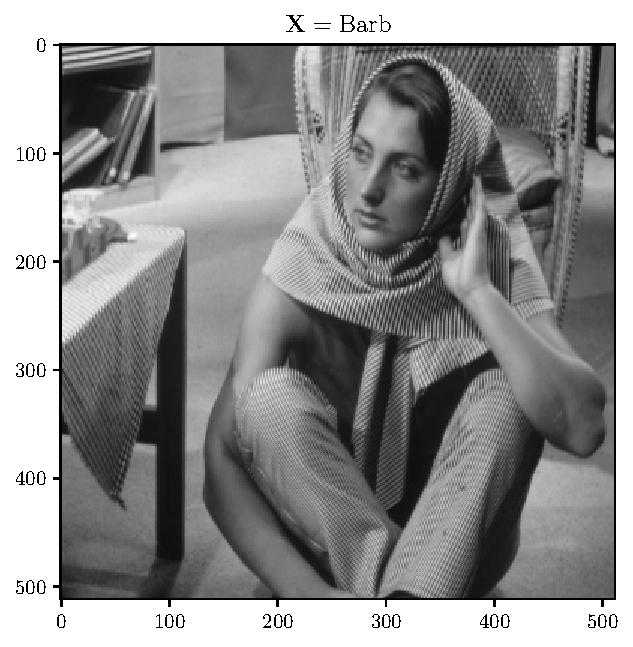
\includegraphics{barb.pdf}} & \href{https://nbviewer.org/github/vicente-gonzalez-ruiz/denoising/blob/main/notebooks/barb_0MMPG.ipynb\#barb_0MMPG}{\includegraphics{barb_0MMPG.pdf}} \\
      \href{https://nbviewer.org/github/vicente-gonzalez-ruiz/denoising/blob/main/notebooks/barb_averaging.ipynb\#barb_averaging}{\includegraphics{barb_averaging.pdf}} & \href{https://nbviewer.org/github/vicente-gonzalez-ruiz/denoising/blob/main/notebooks/barb_averaging_PSNR.ipynb\#barb_averaging_PSNR}{\includegraphics{barb_averaging_PSNR.pdf}}
    \end{tabular}
  }
  \caption{Increase of the SNR as a function of the number of noisy
    instances used in MNI. The clean image is shown on the top-left,
    and a noisy instance on the top-right. On the bottom-left, the
    denoised NMI image, and on the bottom-right the progression of the
    SNR as a function of $I$ and the level of
    noise.\label{fig:MNI_0MMPG}}
\end{figure}

\begin{comment}
%{{{

Fig.~\ref{fig:0MAUN} shows an
example of how zero-mean uniform noise is cancelled by averaging.
  
  \begin{figure}
    \centering
    \resizebox{1.0\textwidth}{!}{
      \renewcommand{\arraystretch}{0.0} % Adjust row spacing in the table
      \setlength{\tabcolsep}{0ex}      % Adjust column spacing in the table    
      \begin{tabular}{cc}
        \href{https://nbviewer.org/github/vicente-gonzalez-ruiz/denoising/blob/main/figs/averaging_denoising.ipynb\#Display-Barb}{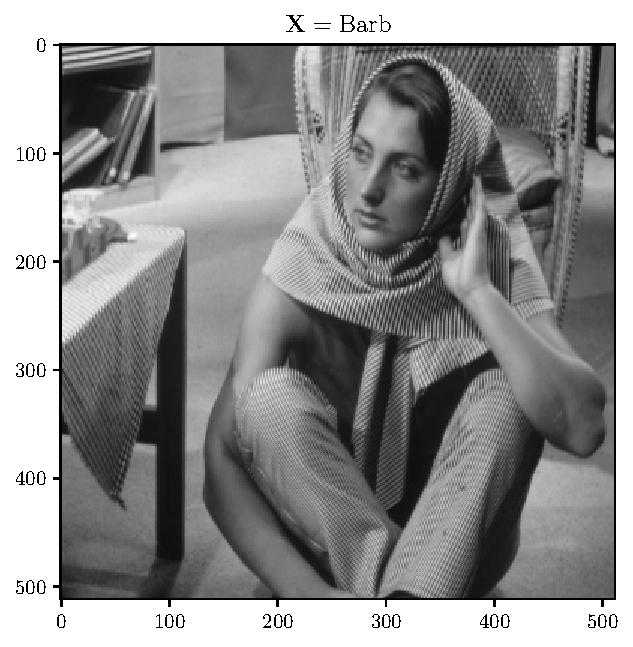
\includegraphics{barb}} & \href{https://nbviewer.org/github/vicente-gonzalez-ruiz/denoising/blob/main/figs/averaging_denoising.ipynb\#0MAUN_barb}{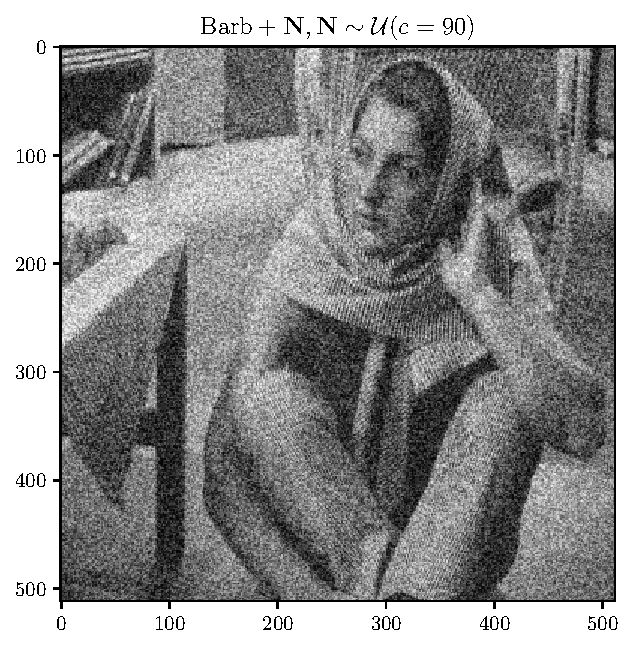
\includegraphics{0MAUN_barb}} \\
        \href{https://nbviewer.org/github/vicente-gonzalez-ruiz/denoising/blob/main/figs/averaging_denoising.ipynb\#denoised_0MAUN_barb}{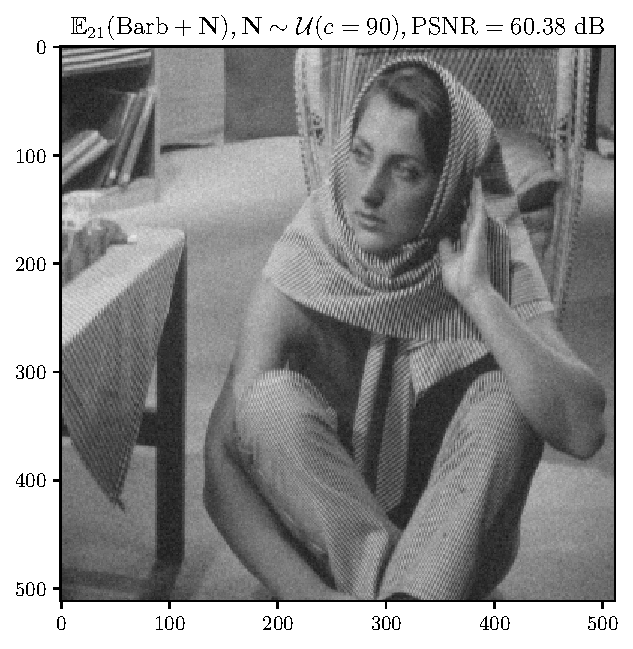
\includegraphics{denoised_0MAUN_barb}} & \href{https://nbviewer.org/github/vicente-gonzalez-ruiz/denoising/blob/main/figs/averaging_denoising.ipynb\#PSNR_0MAUN_barb}{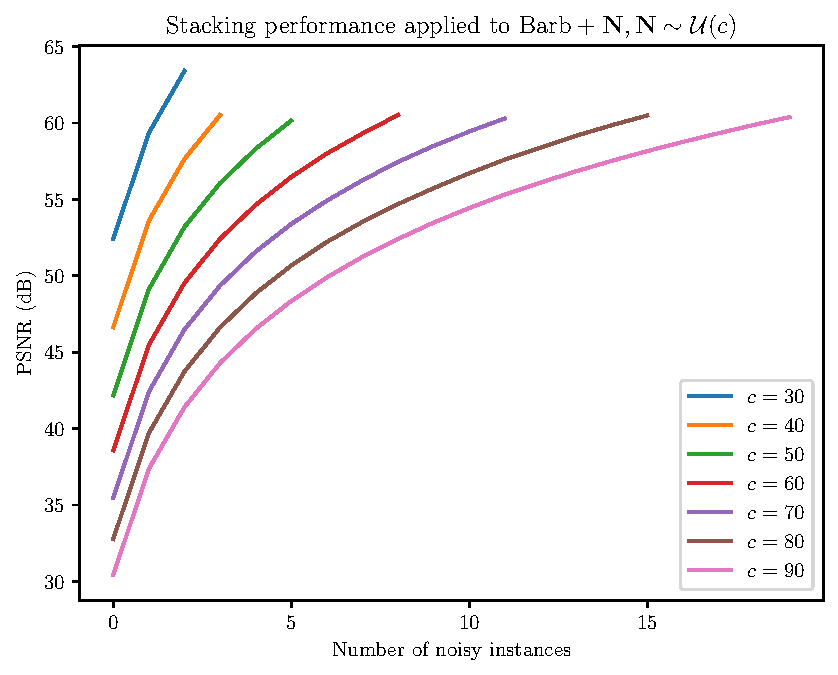
\includegraphics{PSNR_0MAUN_barb}}
      \end{tabular}
    }
    \caption{Effect of zero-mean additive uniform noise in an image
      and how averaging can be used to reduced by averaging. The clean
      image of Barb is shown on the top left, and a noisy version on
      the top right. On to bottom, the left image shows a denoised
      version after averaging and the right graph shows the performance
      of the averaging process for different levels of
      noise.\label{fig:0MAUN}}
  \end{figure}

 Fig.~\ref{fig:0MAGN} shows an
  example of how zero-mean Gaussian noise is cancelled by averaging.

  \begin{figure}
    \centering
    \resizebox{1.0\textwidth}{!}{
      \renewcommand{\arraystretch}{0.0} % Adjust row spacing in the table
      \setlength{\tabcolsep}{0ex}      % Adjust column spacing in the table    
      \begin{tabular}{cc}
        \href{https://nbviewer.org/github/vicente-gonzalez-ruiz/denoising/blob/main/figs/averaging_denoising.ipynb\#barb}{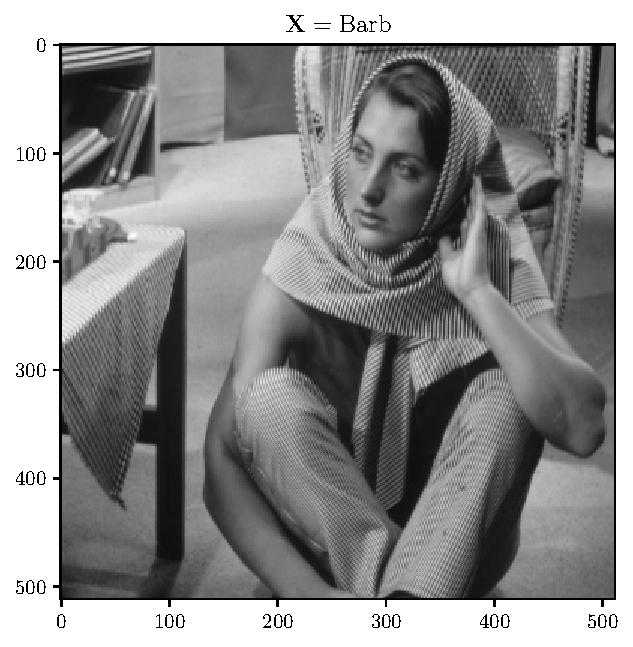
\includegraphics{barb}} & \href{https://nbviewer.org/github/vicente-gonzalez-ruiz/denoising/blob/main/figs/averaging_denoising.ipynb\#0MAGN_barb}{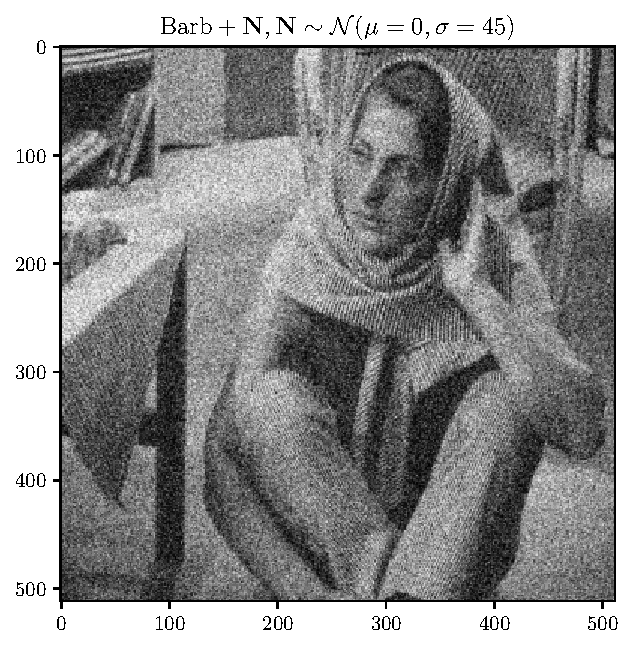
\includegraphics{0MAGN_barb}} \\
        \href{https://nbviewer.org/github/vicente-gonzalez-ruiz/denoising/blob/main/figs/averaging_denoising.ipynb\#denoised_0MAGN_barb}{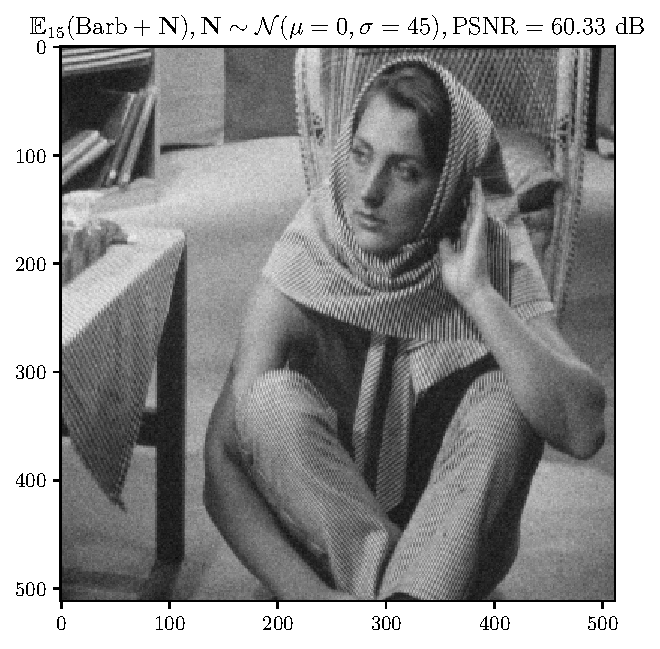
\includegraphics{denoised_0MAGN_barb}} & \href{https://nbviewer.org/github/vicente-gonzalez-ruiz/denoising/blob/main/figs/averaging_denoising.ipynb\#PSNR_0MAGN_barb}{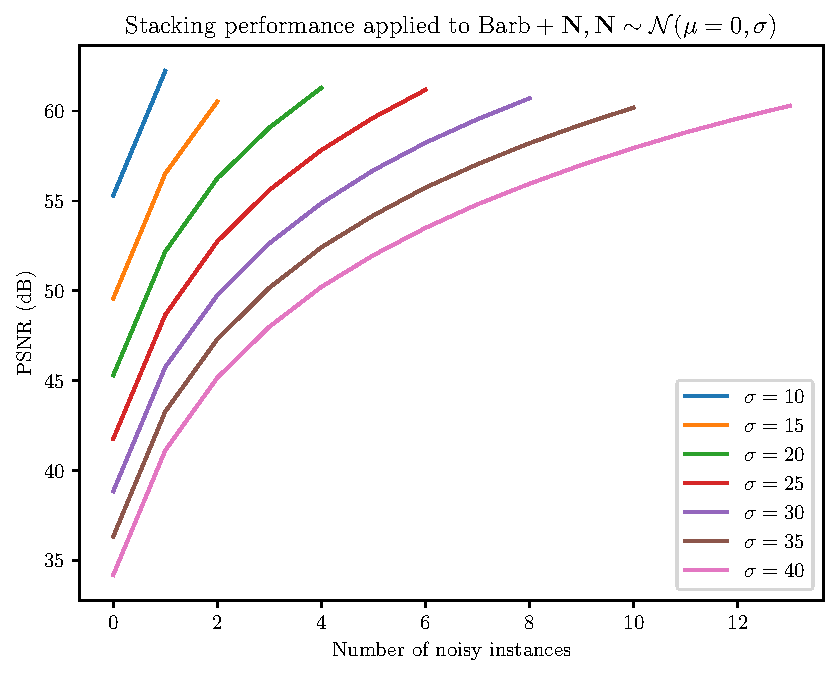
\includegraphics{PSNR_0MAGN_barb}}
      \end{tabular}
    }
    \caption{Effect of zero-mean additive Gaussian noise in an image
      and how averaging can be used to reduced by averaging. The clean
      image of Barb is shown on the top left, and a noisy version on
      the top right. On to bottom, the left image shows a denoised
      version after averaging and the right graph shows the performance
      of the averaging process for different levels of
      noise.\label{fig:0MAGN}}
  \end{figure}

  Fig.~\ref{fig:0MMGN} shows an example of
  how zero-mean Gaussian noise is cancelled by averaging.

  \begin{figure}
    \centering
    \resizebox{1.0\textwidth}{!}{
      \renewcommand{\arraystretch}{0.0} % Adjust row spacing in the table
      \setlength{\tabcolsep}{0ex}      % Adjust column spacing in the table    
      \begin{tabular}{cc}
        \href{https://nbviewer.org/github/vicente-gonzalez-ruiz/denoising/blob/main/figs/averaging_denoising.ipynb\#barb}{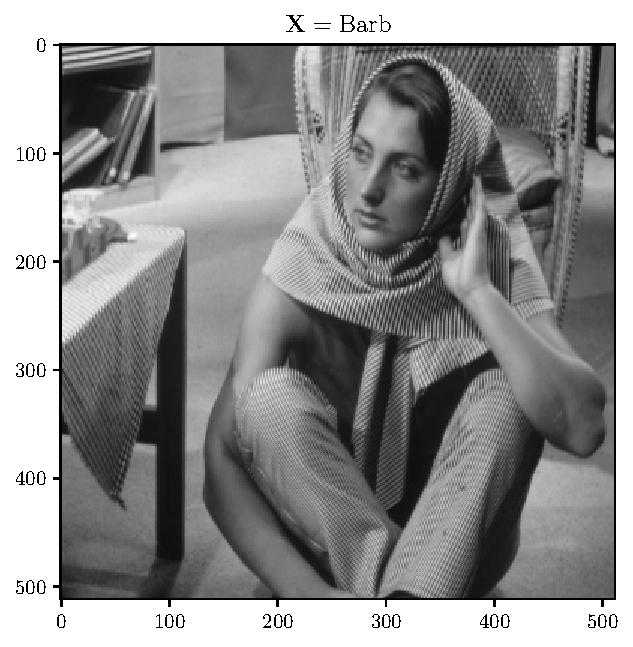
\includegraphics{barb}} & \href{https://nbviewer.org/github/vicente-gonzalez-ruiz/denoising/blob/main/figs/averaging_denoising.ipynb\#0MMGN_barb}{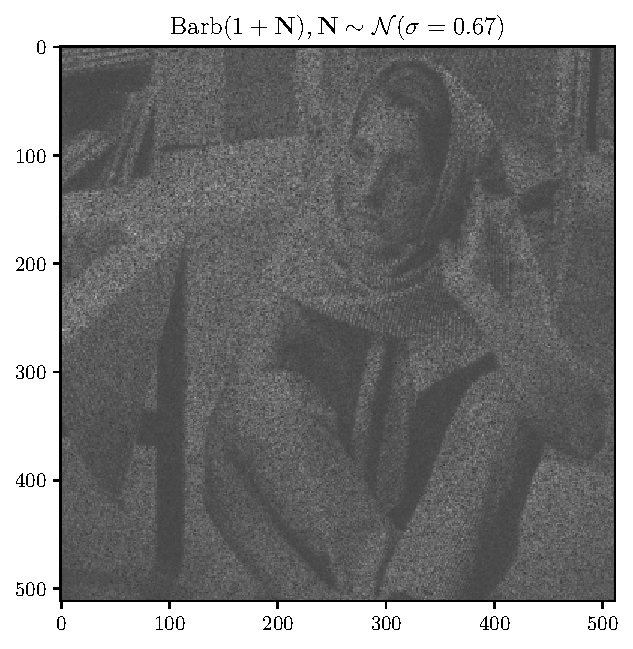
\includegraphics{0MMGN_barb}} \\
        \href{https://nbviewer.org/github/vicente-gonzalez-ruiz/denoising/blob/main/figs/averaging_denoising.ipynb\#denoised_0MMGN_barb}{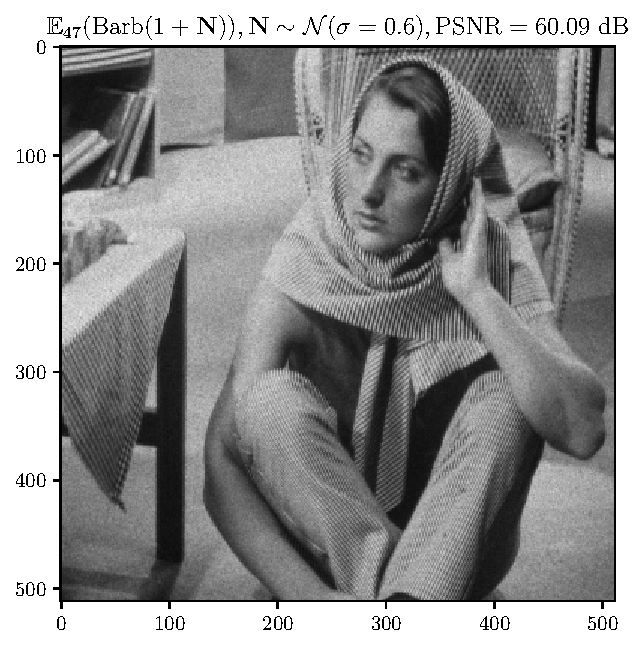
\includegraphics{denoised_0MMGN_barb}} & \href{https://nbviewer.org/github/vicente-gonzalez-ruiz/denoising/blob/main/figs/averaging_denoising.ipynb\#PSNR_0MMGN_barb}{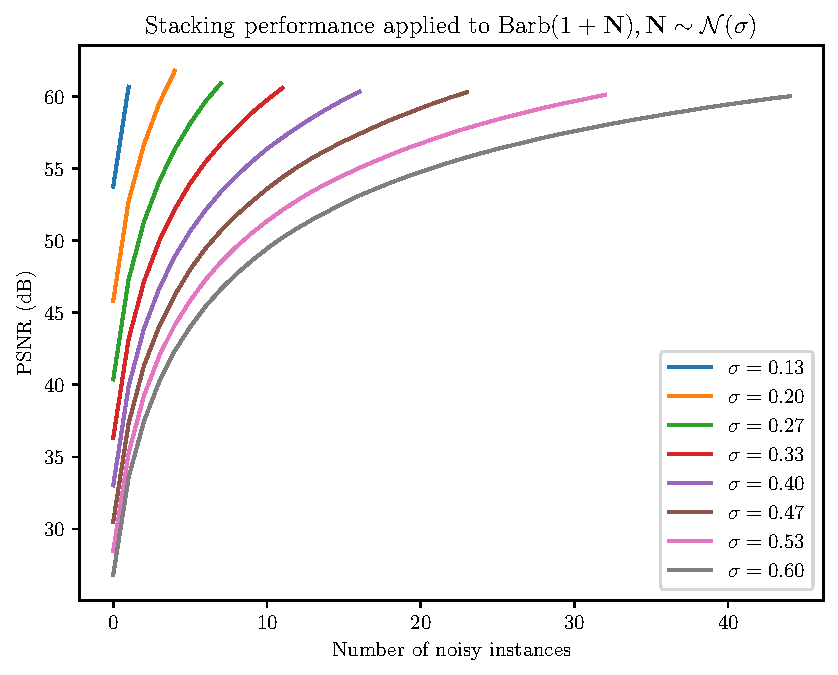
\includegraphics{PSNR_0MMGN_barb}}
      \end{tabular}
    }
    \caption{Effect of zero-mean multiplicative Gaussian noise in an
      image and how averaging can be used to reduced by averaging. The
      clean image of Barb is shown on the top left, and a noisy
      version on the top right. On to bottom, the left image shows a
      denoised version after averaging and the right graph shows the
      performance of the averaging process for different levels of
      noise.\label{fig:0MMGN}}
  \end{figure}

 Fig.~\ref{fig:Rayleigh}
  shows an example of how Rayleigh noise is cancelled by averaging.

  \begin{figure}
    \centering
    \resizebox{1.0\textwidth}{!}{
      \renewcommand{\arraystretch}{0.0} % Adjust row spacing in the table
      \setlength{\tabcolsep}{0ex}      % Adjust column spacing in the table    
      \begin{tabular}{cc}
        \href{https://nbviewer.org/github/vicente-gonzalez-ruiz/denoising/blob/main/figs/averaging_denoising.ipynb\#barb}{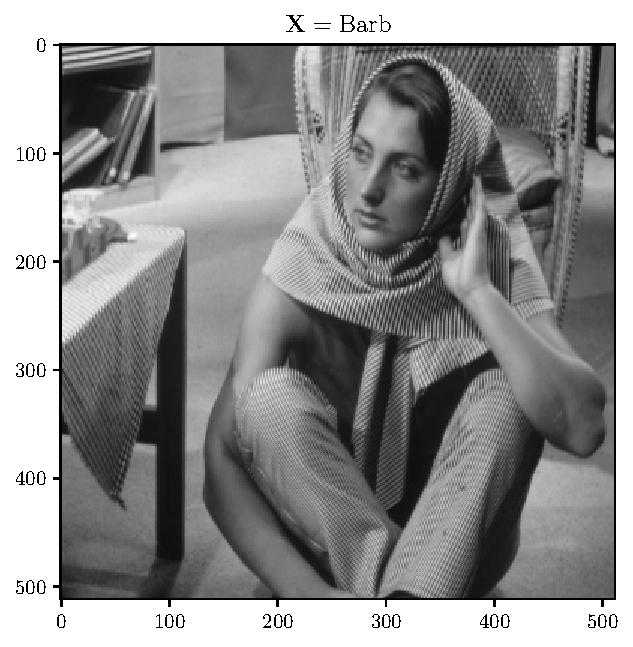
\includegraphics{barb}} & \href{https://nbviewer.org/github/vicente-gonzalez-ruiz/denoising/blob/main/figs/averaging_denoising.ipynb\#Rayleigh_barb}{\includegraphics{Rayleigh_barb}} \\
        \href{https://nbviewer.org/github/vicente-gonzalez-ruiz/denoising/blob/main/figs/averaging_denoising.ipynb\#denoised_Rayleigh_barb}{\includegraphics{denoised_Rayleigh_barb}} & \href{https://nbviewer.org/github/vicente-gonzalez-ruiz/denoising/blob/main/figs/averaging_denoising.ipynb\#PSNR_Rayleigh_barb}{\includegraphics{PSNR_Rayleigh_barb}}
      \end{tabular}
    }
    \caption{Effect of Rayleigh noise in an image and how averaging can
      be used to reduced by averaging. The clean image of Barb is shown
      on the top left, and a noisy version on the top right. On to
      bottom, the left image shows a denoised version after averaging
      and the right graph shows the performance of the averaging
      process for different levels of noise.\label{fig:Rayleigh}}
  \end{figure}

  Fig.~\ref{fig:Poisson} shows an example of how Poisson noise is
  cancelled by averaging.

  \begin{figure}
    \centering
    \resizebox{1.0\textwidth}{!}{
      \renewcommand{\arraystretch}{0.0} % Adjust row spacing in the table
      \setlength{\tabcolsep}{0ex}      % Adjust column spacing in the table    
      \begin{tabular}{cc}
        \href{https://nbviewer.org/github/vicente-gonzalez-ruiz/denoising/blob/main/figs/averaging_denoising.ipynb\#barb}{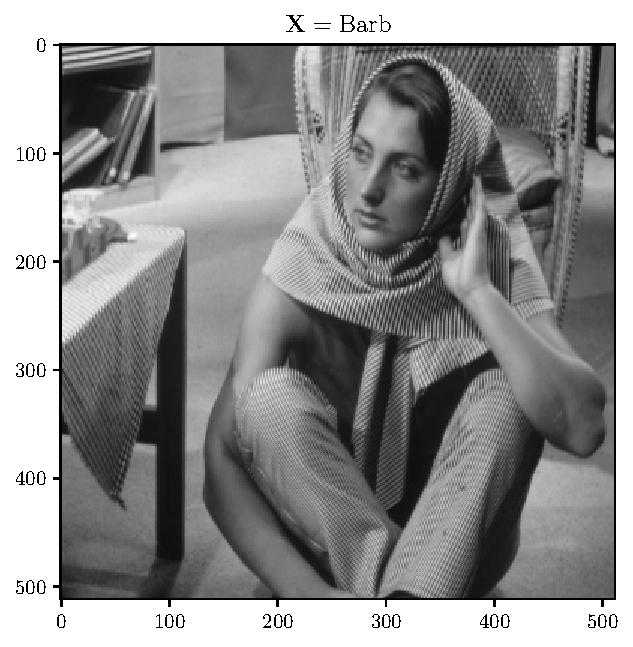
\includegraphics{barb}} & \href{https://nbviewer.org/github/vicente-gonzalez-ruiz/denoising/blob/main/figs/averaging_denoising.ipynb\#Poisson_barb}{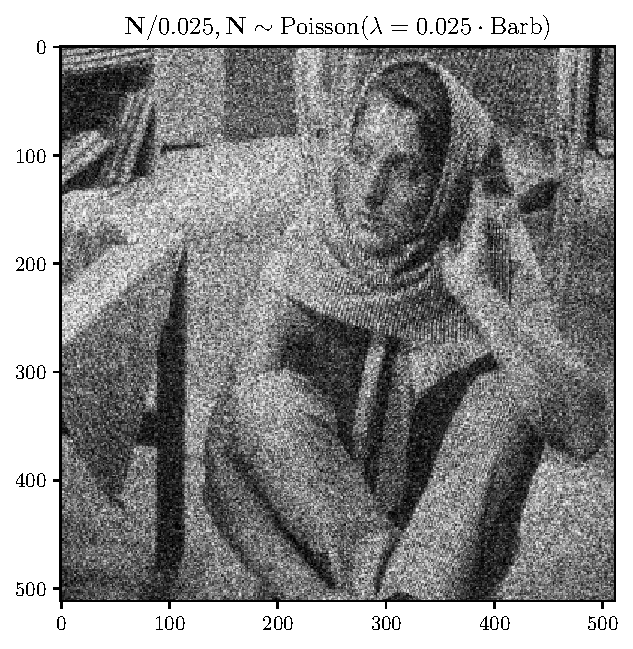
\includegraphics{Poisson_barb}} \\
        \href{https://nbviewer.org/github/vicente-gonzalez-ruiz/denoising/blob/main/figs/averaging_denoising.ipynb\#denoised_Poisson_barb}{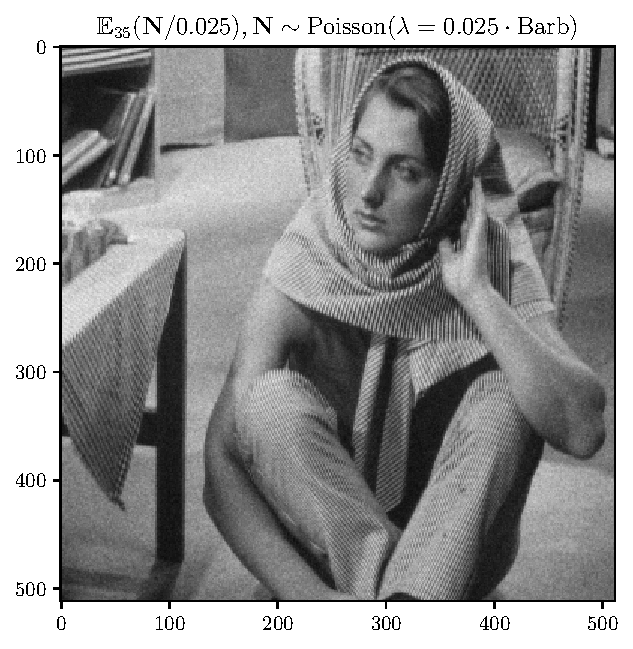
\includegraphics{denoised_Poisson_barb}} & \href{https://nbviewer.org/github/vicente-gonzalez-ruiz/denoising/blob/main/figs/averaging_denoising.ipynb\#PSNR_Poisson_barb}{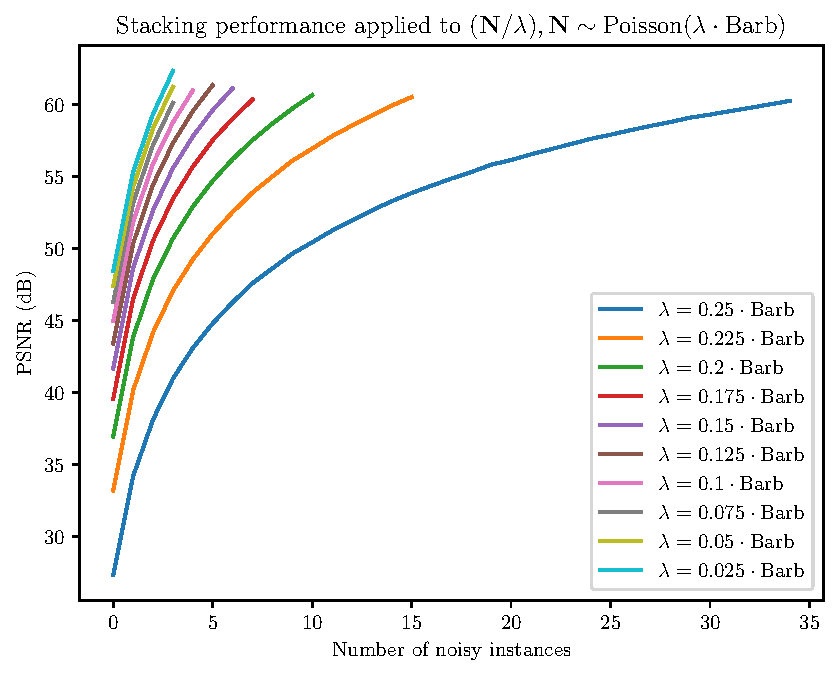
\includegraphics{PSNR_Poisson_barb}}
      \end{tabular}
    }
    \caption{Effect of Poisson noise in an image and how averaging can
      be used to reduced by averaging. The clean image is shown
      on the top left, and a noisy version on the top right. On the
      bottom, the left image shows a denoised version after averaging
      and the right graph shows the performance of the averaging
      process for different levels of noise.\label{fig:Poisson}}
  \end{figure}

%}}}
\end{comment}

%}}}

%}}}
